% Author: Till Tantau
% Source: The PGF/TikZ manual

\documentclass[14pt,border=10pt]{standalone}
\usepackage{tikz}
%\usepackage[american]{circuitikz}
\usepackage[]{circuitikz}
\usepackage{textcomp}

%\usetikzlibrary{shapes,arrows}
\usetikzlibrary{arrows,automata}
%\usepackage[latin1]{inputenc}
% Utilizamos el paquete para utilizar espanol
%\usepackage[spanish,es-noshorthands]{babel}
% Utilizamos un paquete para gestionar los acentos
% y las eoes
%\usepackage[utf8]{inputenc}

\begin{document}
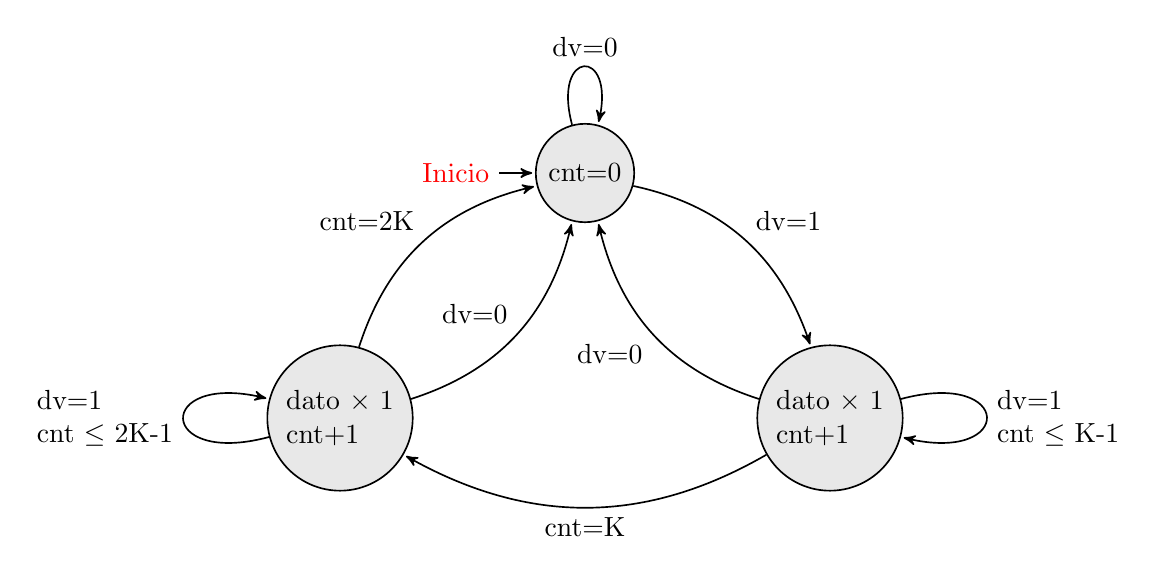
\begin{tikzpicture}[initial text = \textcolor{red}{Inicio},->,>=stealth',shorten >=1pt,auto,node distance=4.4cm,
                    semithick]
  %\tikzstyle{every state}=[fill=red,draw=none,text=white]
	\tikzstyle{every state}=[fill={rgb:black,1;white,10}]

  \node[initial,state] (A)                    {cnt=0};
  \node[state]         (B) [align=left,below right of=A] {dato $\times$ 1 \\ cnt+1};
  \node[state]         (C) [align=left,below left of=A] {dato $\times$ 1 \\ cnt+1};

  \path (A) edge [loop above] node {dv=0} (A)
				(A) edge [bend left]  node {dv=1} (B)
				(B) edge [bend left]  node {dv=0} (A)
				(B)	edge [bend left]  node {cnt=K} (C)
        (B) edge [loop right,align=left] node {dv=1 \\ cnt $\le$ K-1 } (B)
        %    edge              node {0,1,L} (C)
        (C) edge [loop left,align=left] node {dv=1 \\ cnt $\le$ 2K-1 } (C)
				(C) edge [bend left]  node {cnt=2K} (A)
				(C) edge [bend right] node {dv=0} (A);
        %    edge [bend left]  node {1,0,R} (E)
       % (D) edge [loop below] node {1,1,R} (D)
        %    edge              node {0,1,R} (A)
        %(E) edge [bend left]  node {1,0,R} (A);
\end{tikzpicture}

\end{document}
